\begin{figure}[tbp]
\begin{center}
\includegraphics[width=0.48\textwidth]{Cl_sn_z1z2.eps}
\end{center}
\vspace{-0.7cm}
\caption{(Top) Relative strength of kSZ signal, within a box of $\Delta \chi=1200 Mpc/h$. 
    (Bottom) predicted S/N, assuming Planck noise, $\Delta l/l=0.1$, $f_{sky}=0.8$. 
}
\label{fig:sn}
\end{figure}
%In real surveys, when we calculate the cross angular power spectrum $C_l$ between reconstructed kSZ signals and CMB measurements, we will have to face statistical errors. 
%They can be approximated as:
We use the statistical error to estimate the S/N ratio for real surveys. 
Taking into account the contamination from primary CMB and facility noises, it can be approximated as:
%\begin{eqnarray}
 %   \frac{\Delta C_l}{C_l}\simeq \frac{1}{r\sqrt{(2l+1)\Delta l f_{sky}}}\sqrt{\frac{C_l^{\mr{CMB}}+C_l^{kSZ}+C_l^{\mr{CMB},N}}{C_l^{kSZ,\Delta z}}(1+\frac{C^N_{\hat \Theta}}{C_{\hat \Theta}})}\,
%\end{eqnarray}
\begin{eqnarray}
    \frac{\Delta C_l}{C_l}\simeq \frac{1}{r\sqrt{(2l+1)\Delta l f_{sky}}}\sqrt{\frac{C_l^{\mr{CMB}}+C_l^{kSZ}+C_l^{\mr{CMB},N}}{C_l^{kSZ,\Delta z}}}\,
\end{eqnarray}
Where $C_l^{CMB}$ is the angular powerspectrum of primary CMB; 
$C_l^{CMB,N}$ indicates the facility noises; 
$C_l^{kSZ,\Delta z}$ is the kSZ signal from a certain redshift bin; 
r is the correlation coefficients we get; 
$f_{sky}$ is the percent of sky area covered by both surveys.

In our case, we calculate $C_l^{CMB}$ from CAMB \cite{CAMB}. 
We use Planck 2015 results \cite{Planck2015} at 217GHz to estimate $C_l^{CMB,N}$.
$C_l^{CMB,N}=(\sigma_{p,T}\theta_{FWHM})^2W_l^{-2}$;  
where $\sigma_{p,T}=8.7\mu K_{CMB}$ is Sensitivity per beam solid angle, 
$\theta_{FWHM}\sim 5'$ is the effective beam FWHM, 
$W_l=exp[-l(l+1)/2l^2_{beam}]$ is the smoothing window function, 
with $l_{beam}=\sqrt{8\ln2}/\theta_{FWHM}$. 
We choose $f_{sky}=0.8$, since it is feasible for 21cm intensity mapping to survey large sky areas. 
We choose $\Delta l/l=0.1$. 
And for $C_l^{kSZ,\Delta z}$, we choose two bins of size 1200 Mpc/h, centered at redshift 1,2 respectively.

In Fig.\ref{fig:sn}, we plot the S/N level for the two redshift bins. 
The S/N will exceeds 3 from $l\sim 500-3000$. 

Since we only use the correlation calculated from tidal reconstructed field, the S/N shall be higher for z=2  
combining tidal reconstructed field and foreground substracted field. 
Moreover, since $C_l^{kSZ}$ is relatively flat, 
it is possible to bin it into larger $\Delta l$. 
eg. \cite{Hill16} choose $\Delta l=200$, and this will yield better S/N for $l<2000$ in Fig.\ref{fig:sn}.

What's more, Planck's noise level is far from ideal. If we consider the case of 4th generation facilities, there will also be a giant leap for S/N at large l. 
However, in that case, we have to have accurate substraction for CMB lensing, 
when primary CMB dims out.
